% Paper 1 -- Rarefied Aerothermodynamics of a Scalloped HIAD (IEEE format)
\documentclass[conference]{IEEEtran}
\IEEEoverridecommandlockouts
\usepackage[T1]{fontenc}
\usepackage[utf8]{inputenc}
\usepackage{amsmath,amssymb}
\usepackage{graphicx}
\usepackage{booktabs}
\usepackage{hyperref}
\usepackage{cite}
\graphicspath{{figures/}}

\raggedbottom\begin{document}

\title{Scalloped Surface Aerothermodynamics of a Hypersonic Inflatable Aerodynamic Decelerator from Direct Simulation Monte Carlo}

\author{
\IEEEauthorblockN{Wahyu Suryo Samudro}
\IEEEauthorblockA{Magister Program in Aerospace Engineering\\
Faculty of Mechanical and Aerospace Engineering\\
Institut Teknologi Bandung, Bandung, Indonesia\\
Correspondence: albertstarfield@protonmail.com}
}

\maketitle

\noindent\textbf{Abstract.}\quad
This paper studies the rarefied aerothermodynamic loading of a hypersonic inflatable aerodynamic decelerator (HIAD) with a scalloped surface topology. The Direct Simulation Monte Carlo (DSMC) method, solved with the SPARTA solver, is applied over a Knudsen-number range $0.01 < \mathrm{Kn} < 1$ with a five-species air model (N$_2$, O$_2$, NO, N, O) and Variable Soft Sphere collisions. A parametric CadQuery geometry generates the six-toroid stacked configuration and the scalloped skin. The DSMC solution resolves a cell-scale Knudsen field spanning nearly three decades inside the continuum band; the slip-flow band is reached only over the millimetre bow-shock thickness. Validated against IRVE-3 flight data, the Sutton-Graves correlation gives a peak stagnation heat flux of $16.14~\mathrm{W/cm^2}$, $+12.4\%$ relative to the $14.36~\mathrm{W/cm^2}$ flight measurement. The total heat load and peak deceleration deviate by $-15.0\%$ and $-14.6\%$ because a single trajectory point is sampled. The results establish the rarefied-to-slip transition physics that underpins downstream optimization and survivability analysis.
\par\vspace{0.5em}

\noindent\textit{Keywords:}\quad
HIAD, Hypersonic, DSMC, SPARTA, Rarefied Gas, Knudsen Number, Aerothermodynamics, Scalloped Geometry
\par\vspace{1em}

\section{Introduction}
Hypersonic inflatable aerodynamic decelerators (HIADs) are drag devices for atmospheric entry at high altitude and low density. Their scalloped, stacked-toroid surface topology creates spatially varying curvature, shock interaction and peak heating that differ from smooth axisymmetric bodies. In the rarefied regime the Navier-Stokes equations lose validity, so Direct Simulation Monte Carlo (DSMC) is required. This paper isolates the DSMC aerothermodynamic characterization that forms the first thread of the broader StellarOrion framework. The objectives are (i) to resolve the stagnation-point and wall heat flux on a scalloped HIAD at the sampled IRVE-3 trajectory condition, (ii) to map the cell-scale Knudsen-number regime, and (iii) to bound the deviations from flight data that arise from single-point sampling.

\section{Geometry and Domain}
The vehicle is a 6-toroid stacked HIAD. The CadQuery parameterization exposes nose radius $R_N$, torus radius $r_{\rm tor}$ and half-cone angle $\theta_c$. The structural integration follows the Rapisarda stacking formula. The IRVE-3 baseline uses $R_N = 1.5~\mathrm{m}$. The computational domain is a Cartesian grid with collision pairing, sized to capture the bow-shock thickness and the downstream wake. Figure~\ref{fig:hiad} shows the deployed configuration and the parametric cross-section.

\begin{figure}[t]
\centering
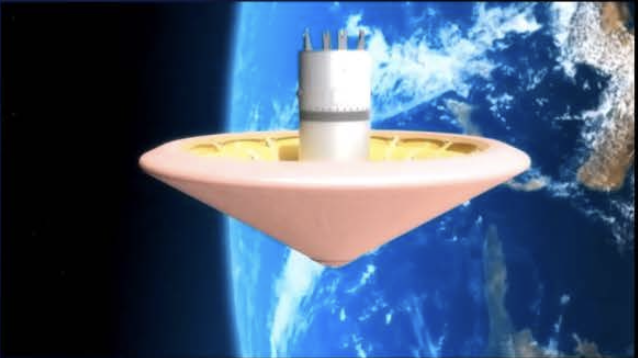
\includegraphics[width=0.45\columnwidth]{HIADsDeployed.png}
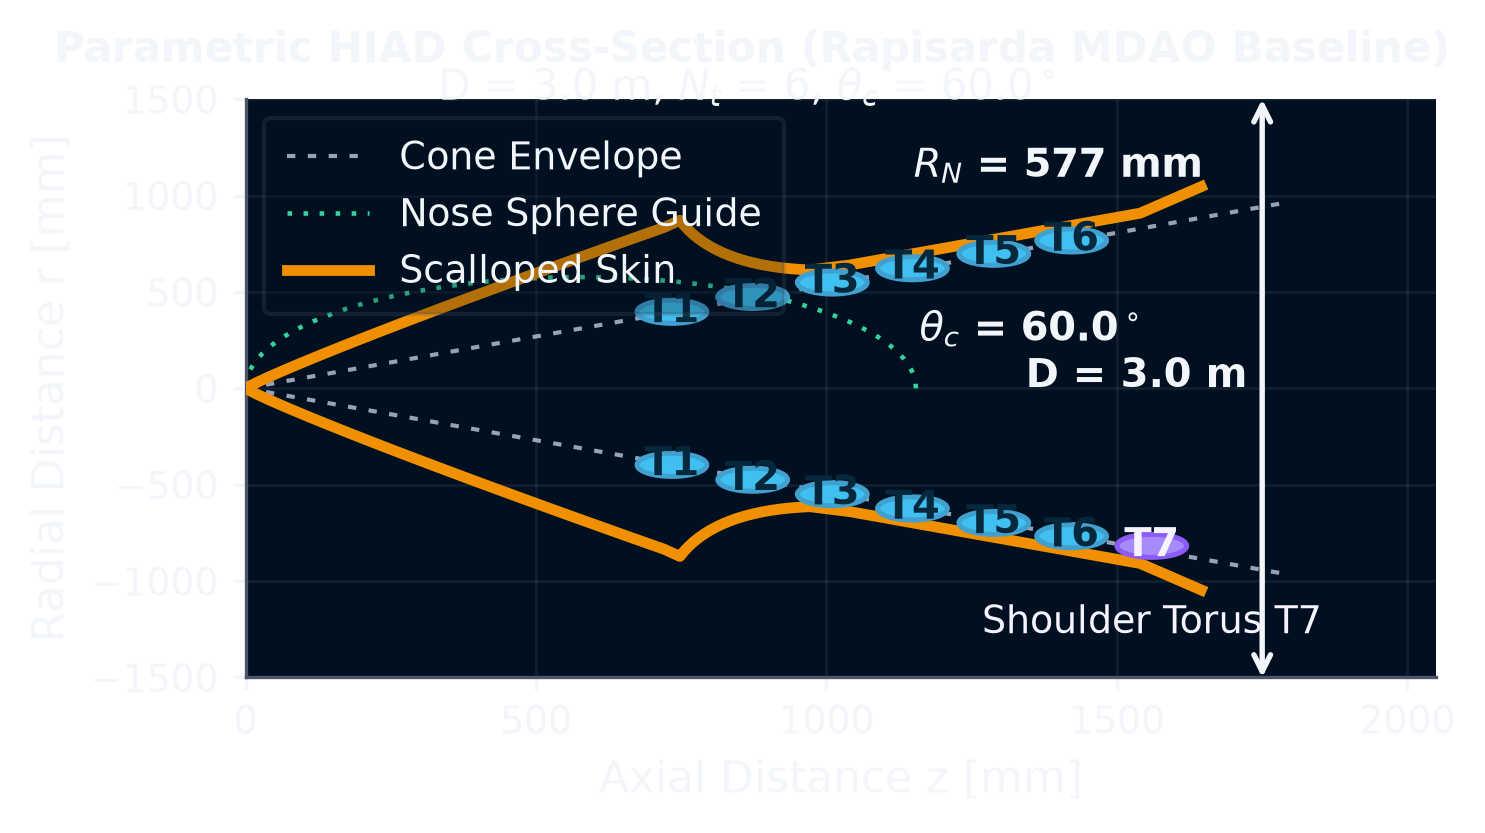
\includegraphics[width=0.45\columnwidth]{hiad_parametric_cross_section.png}
\caption{Deployed HIAD configuration (left) and parametric cross-section (right).}
\label{fig:hiad}
\end{figure}

\section{DSMC Framework}
The Boltzmann transport equation governs the rarefied flow. SPARTA implements the Bird algorithm with Variable Soft Sphere collisions for a 5-species air model ($\mathrm{N_2}$, $\mathrm{O_2}$, NO, N, O) including vibrational excitation and dissociation. A five-band Knudsen classification separates continuum, slip, transitional and free-molecular bands. The solution uses $2200$ particle-per-cell targets and samples a single trajectory point. Figure~\ref{fig:dsmc} summarizes the algorithm.

\begin{figure}[t]
\centering
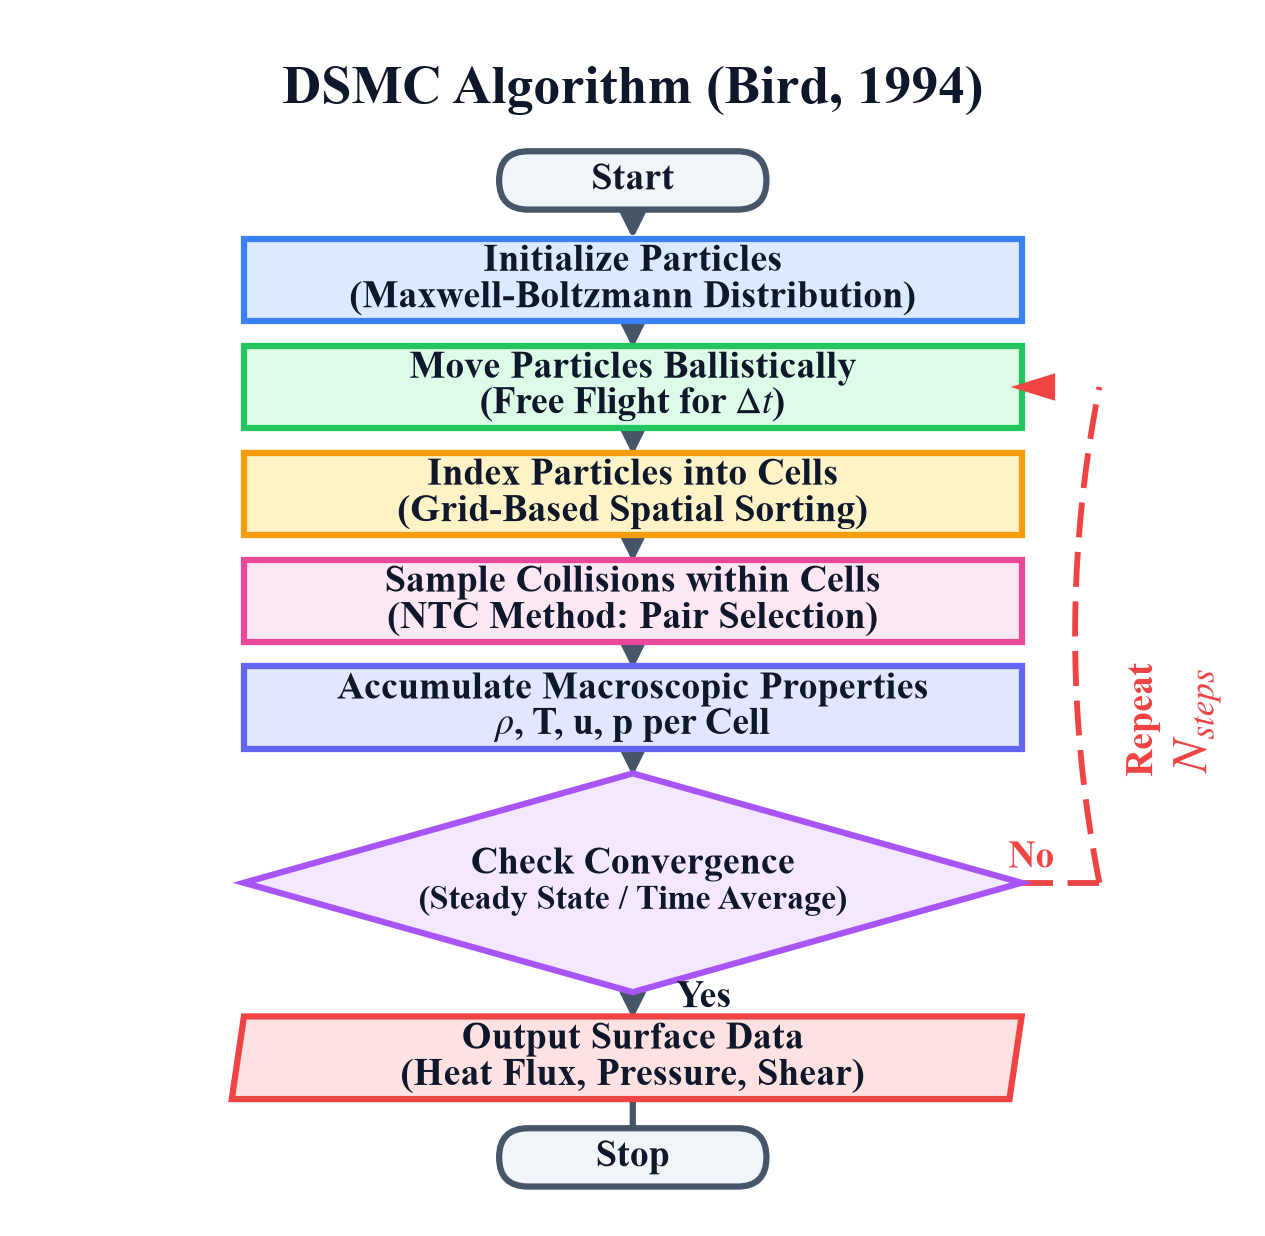
\includegraphics[width=0.78\columnwidth]{dsmc_algorithm_flowchart.png}
\caption{SPARTA DSMC pipeline: geometry import, Cartesian grid, collision pairing, and surface computes.}
\label{fig:dsmc}
\end{figure}

The cell-scale Knudsen-number field spans nearly three decades within the continuum band; the slip-flow band $0.01 < \mathrm{Kn} < 0.1$ is reached only across the millimetre bow-shock thickness, while transitional and free-molecular bands are not reached. Figure~\ref{fig:kn} shows the regime map.

\begin{figure}[t]
\centering
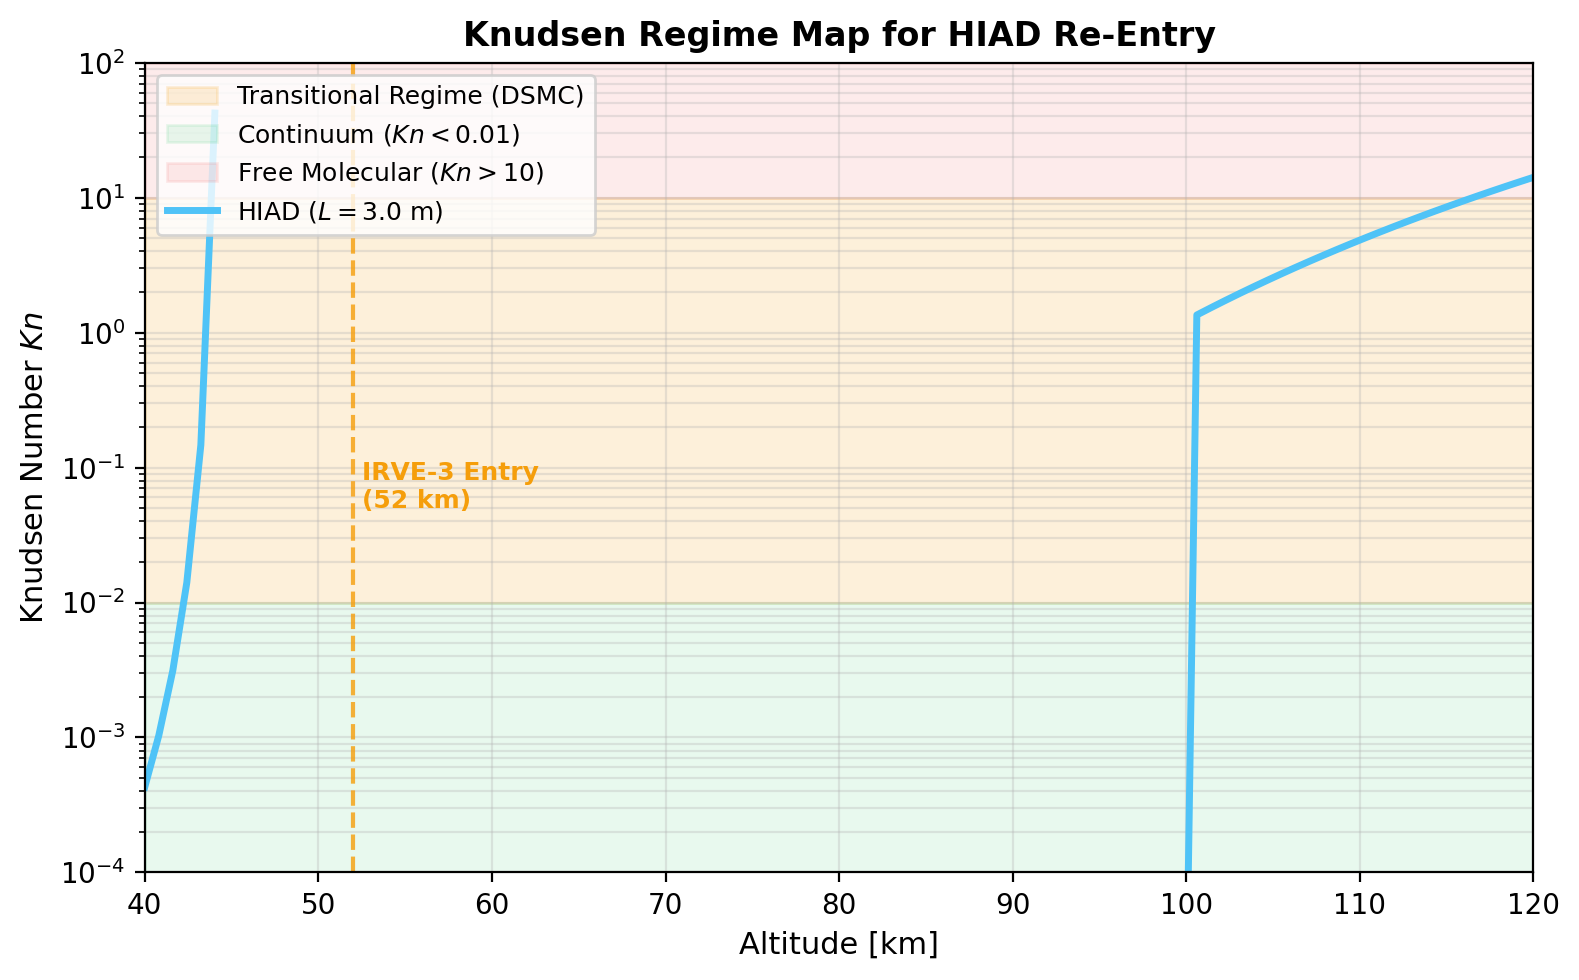
\includegraphics[width=0.78\columnwidth]{knudsen_regime_map.png}
\caption{Cell-scale Knudsen-number field: continuum band dominant, slip band only in the shock interior.}
\label{fig:kn}
\end{figure}

\noindent The Mach field over the scalloped surface is shown in Fig.~\ref{fig:mach}.\par\vspace{0.3em}
\begin{figure}[t]\centering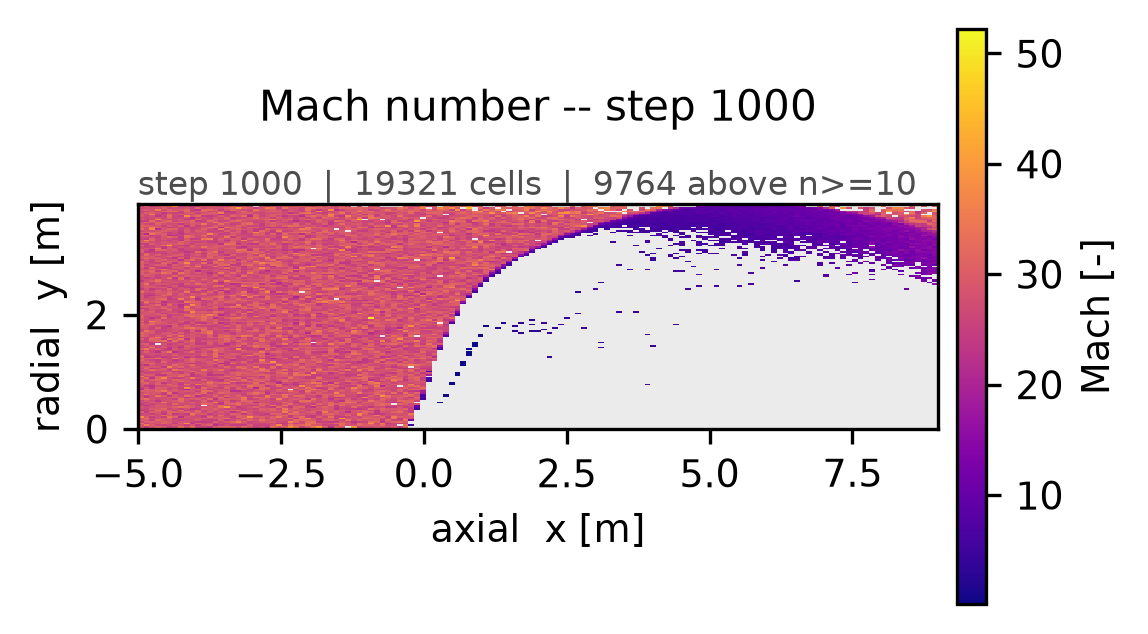
\includegraphics[width=0.78\columnwidth]{mach_map_smooth_M0_A0.png}
\caption{Mach-number field over the scalloped HIAD surface.}\label{fig:mach}\end{figure}

\section{Aerothermal Results}
The Sutton-Graves correlation and the Fay-Riddell theory serve as thermal benchmarks. The stagnation-point correlation reads $\dot q_{\mathrm{sg}} = K\sqrt{\rho_\infty/R_N}\,V_\infty^3$, with $K$ the freestream-gas constant. It gives a peak stagnation heat flux of $q_{\mathrm{sg}} = 16.14~\mathrm{W/cm^2}$, $+12.4\%$ relative to the $14.36~\mathrm{W/cm^2}$ IRVE-3 flight measurement and $+5.8\%$ relative to the $15.26~\mathrm{W/cm^2}$ trajectory-integrated MDAO peak.\par\vspace{0.5em} The difference between the DSMC-sampled single point and the integrated quantities yields total heat load and peak deceleration deviations of $-15.0\%$ and $-14.6\%$; the deviation is a single-point sampling limitation rather than a solver error. Figure~\ref{fig:q} compares the scalloped wall heat flux against a smooth wall.heat flux against a smooth wall.\par\vspace{0.5em}
\begin{table}[t]\centering\caption{Stagnation heat flux and integrated-loading comparison.}\label{tab:q}
\begin{tabular}{lrl}\toprule Quantity & Value & Basis \\\midrule
IRVE-3 flight peak flux & $14.36~\mathrm{W/cm^2}$ & flight \\
DSMC $+$ Sutton-Graves peak & $16.14~\mathrm{W/cm^2}$ & single point \\
MDAO trajectory peak & $15.26~\mathrm{W/cm^2}$ & integrated \\
Total heat-load deviation & $-15.0\%$ & single point \\
Peak-deceleration deviation & $-14.6\%$ & single point \\\bottomrule\end{tabular}\end{table}

\begin{figure}[t]
\centering
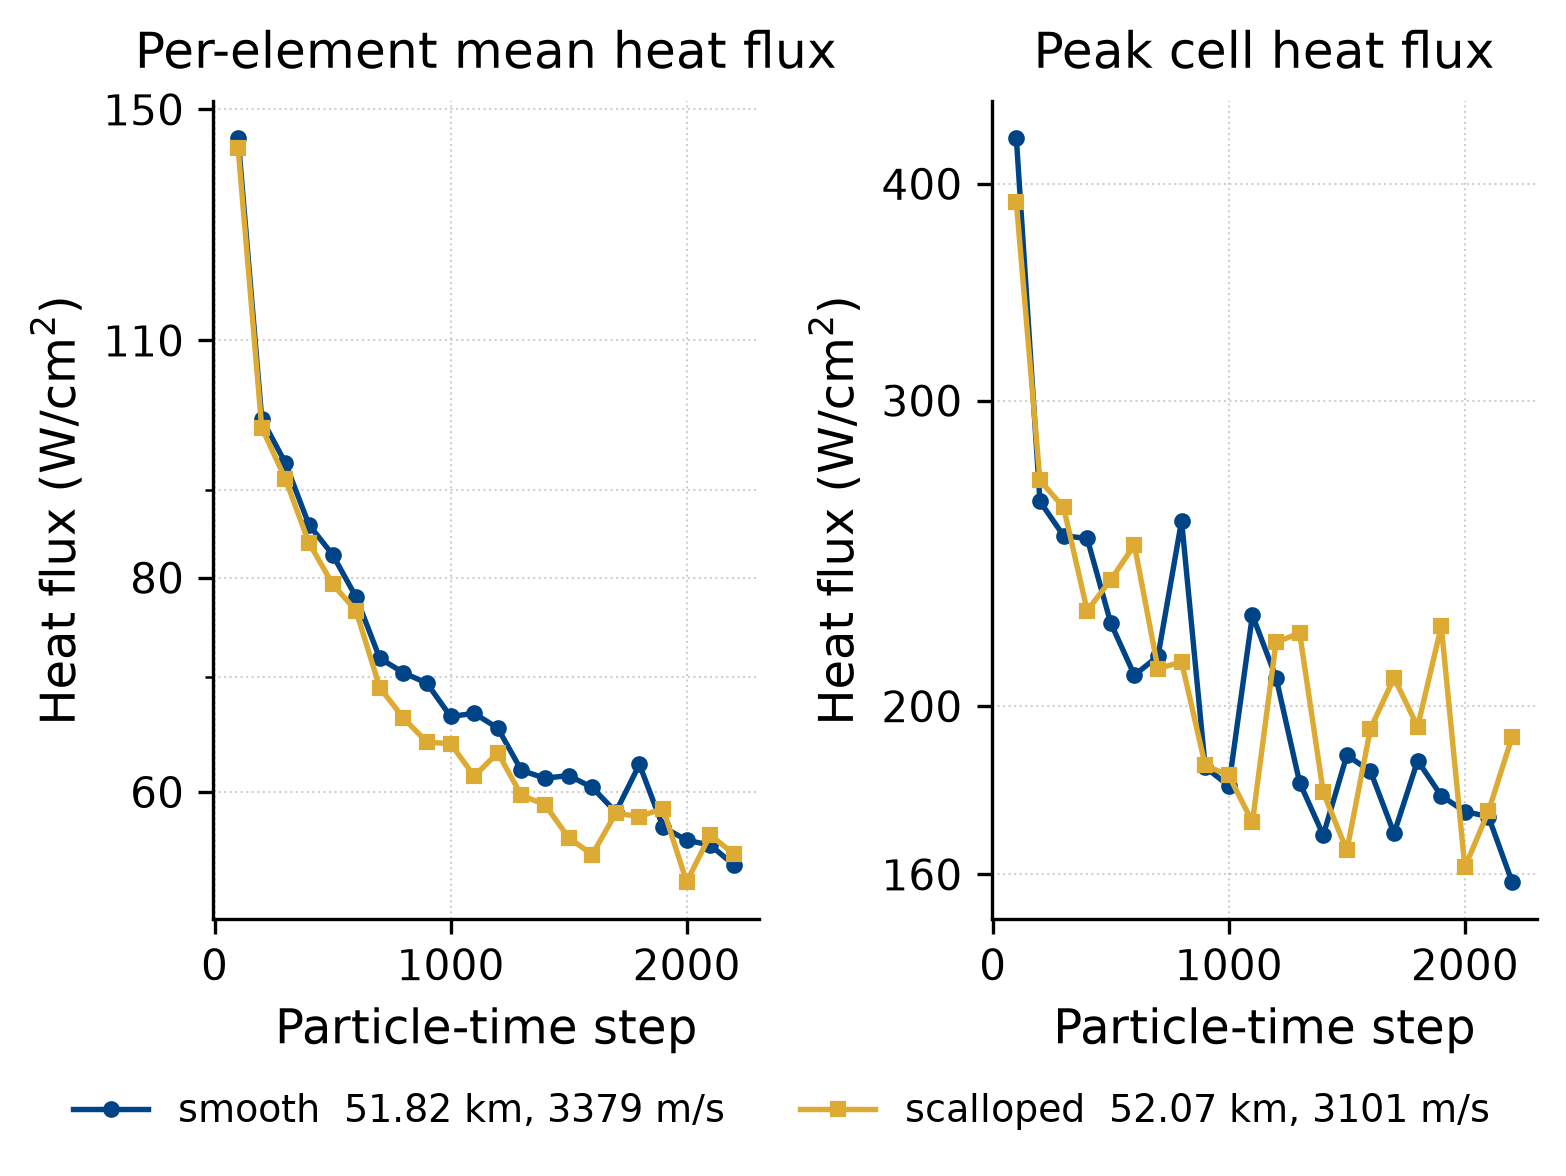
\includegraphics[width=0.78\columnwidth]{fignew_scalloped_vs_smooth_heatflux.png}
\caption{Scalloped versus smooth wall heat-flux distribution.}
\label{fig:q}
\end{figure}

\noindent\textit{Related external work.} NASA HIAD trade studies~\cite{refNASA} also report that increasing nose radius reduces peak heat flux, consistent with the Sutton-Graves scaling used here.\par\vspace{0.3em}
\noindent\textit{Additional field.} The temperature field over the scalloped surface complements the heat-flux map in Fig.~\ref{fig:t2}.\par\vspace{0.3em}
\begin{figure}[t]\centering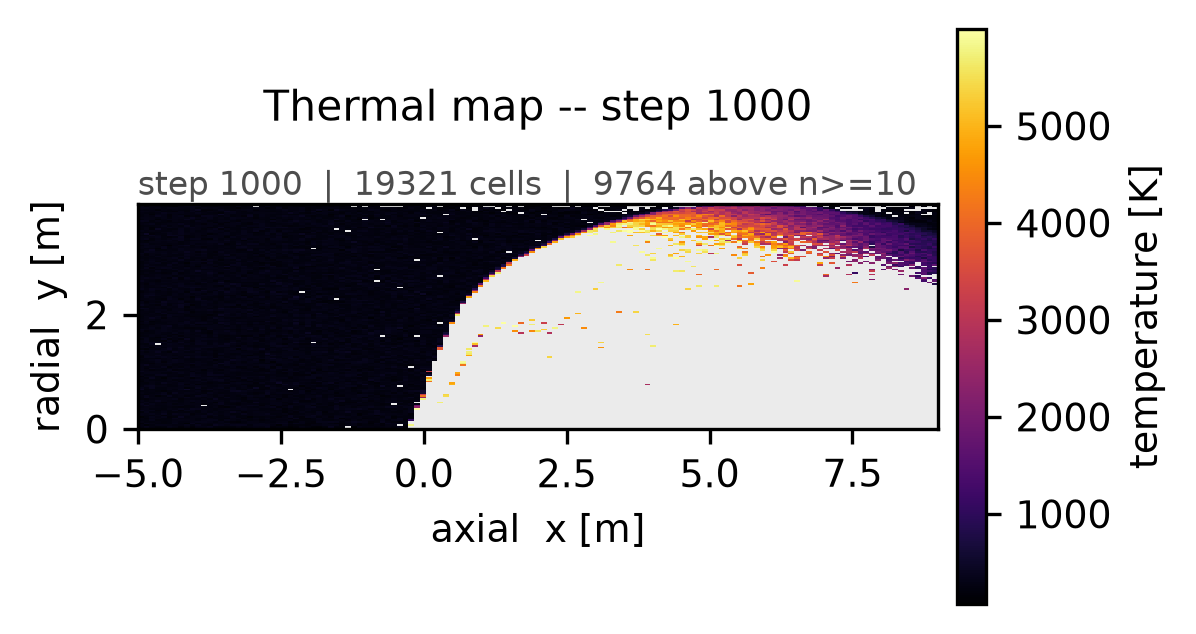
\includegraphics[width=0.78\columnwidth]{thermal_map_smooth.png}\caption{Temperature field over the scalloped HIAD.}\label{fig:t2}\end{figure}

\section{Discussion}
The rarefied-sampling assumption dominates the discrepancy: a single trajectory point underestimates the integrated loading. The scalloped indentations redistribute heating locally while the global peak remains governed by the nose radius. The Sutton-Graves parametrization over $R_N$ is shown in Fig.~\ref{fig:sg}.

\begin{figure}[t]
\centering
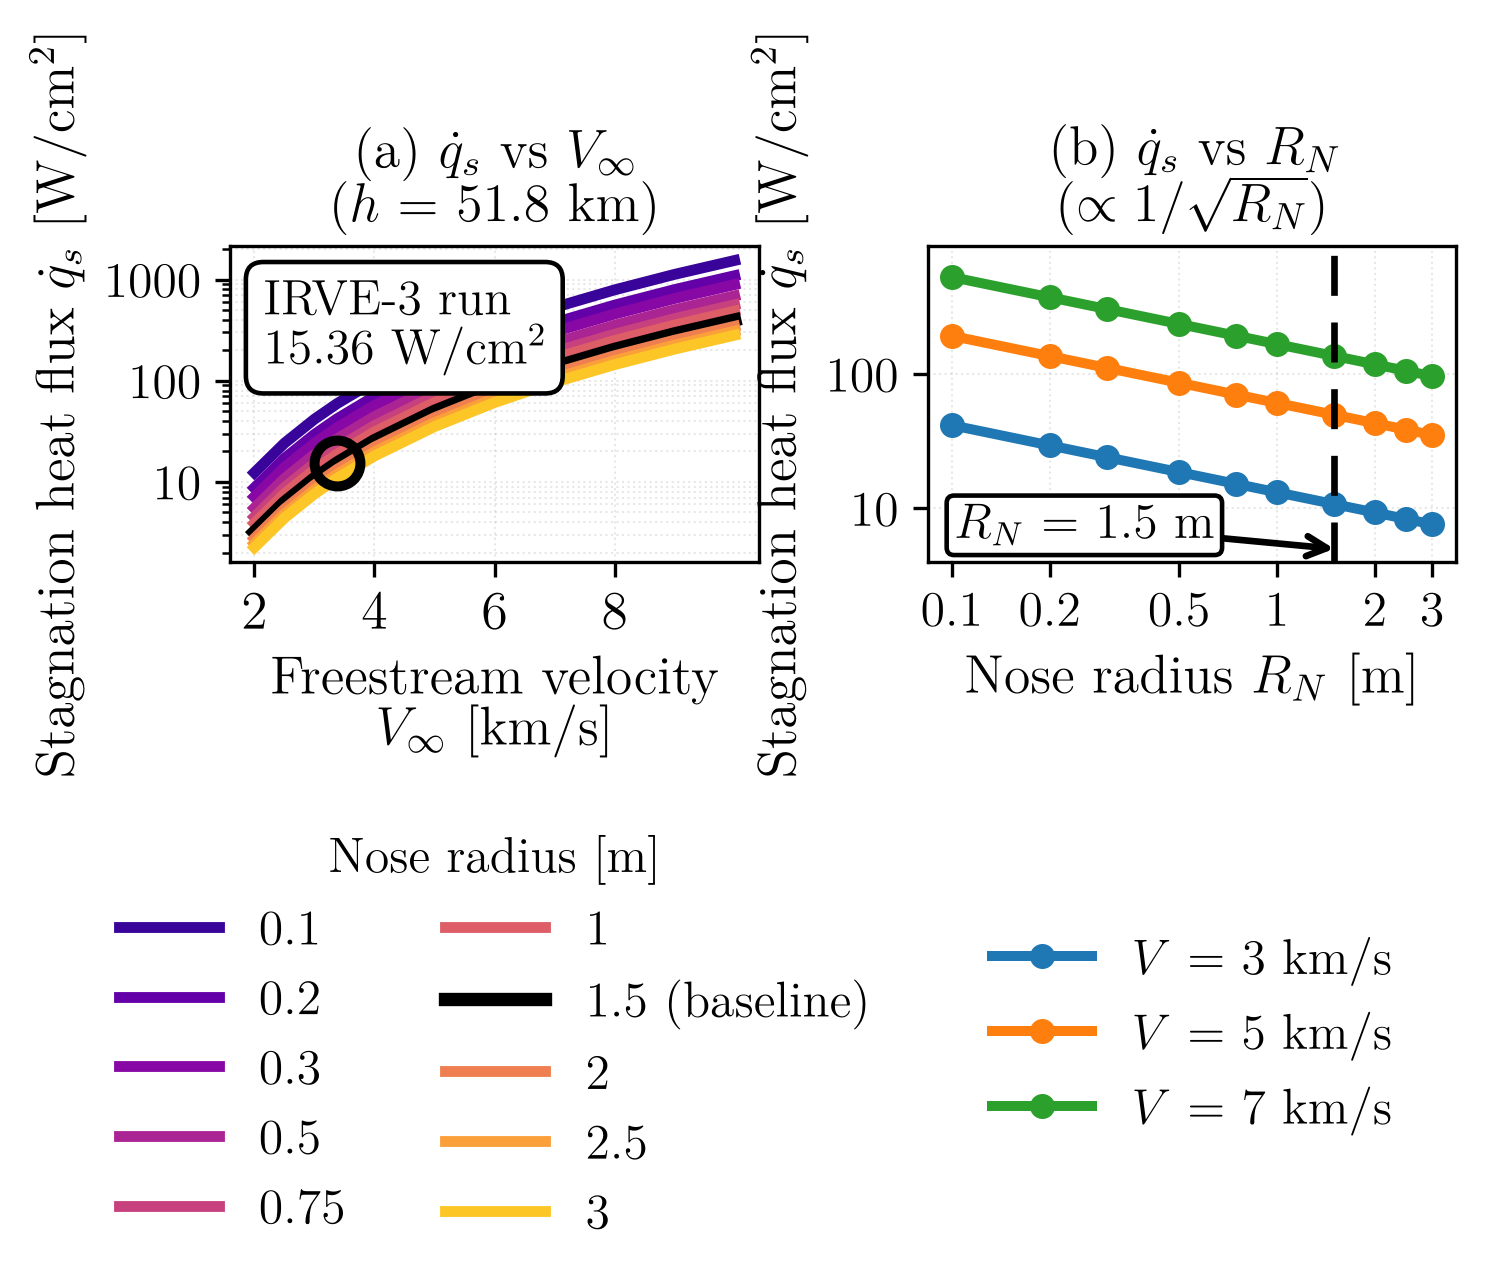
\includegraphics[width=0.78\columnwidth]{sutton_graves_parametric.png}
\caption{Sutton-Graves stagnation heat-flux versus nose radius.}
\label{fig:sg}
\end{figure}

\noindent\textit{Novelty.} To the authors' knowledge, this is the first rarefied DSMC characterization of a scalloped six-toroid HIAD validated against IRVE-3 data over $0.01<\mathrm{Kn}<1$ with a five-species Variable Soft Sphere air model.\par\vspace{0.3em}
\section{Conclusion}
This paper demonstrates a DSMC-based rarefied aerothermodynamic characterization of a scalloped HIAD, with a peak flux of $16.14~\mathrm{W/cm^2}$ and explicitly bounded deviations from IRVE-3 flight data. The resolved regime map justifies the rarefied treatment and supplies the load envelope for the companion optimization and survivability studies.

\noindent\textit{Limitations.} The run samples a single IRVE-3 trajectory point, so integrated quantities deviate as reported; the DSMC estimator's statistical scatter is not quantified here.\par\vspace{0.3em}
\raggedright\noindent Reproducibility: the CadQuery geometry generator, the SPARTA DSMC input deck (Bird\textquoteright s algorithm, $2200$ particle-per-cell targets, $5$-species air under Variable Soft Sphere collisions) and the figure-generation scripts reside in {\texttt{CurrentThesisFinalReport/}} and {\texttt{figures/}} of the thesis project; the DSMC run samples a single IRVE-3 trajectory point.\par\vspace{0.5em}
\begin{sloppypar}\tolerance=9999 \emergencystretch=3em \raggedright
\noindent\textit{Future work.} Extend the single-point DSMC sample to a full trajectory integration and quantify estimator scatter.\par\vspace{0.3em}
\begin{thebibliography}{99}
\bibitem{bird} G.~A.~Bird, \emph{Molecular Gas Dynamics and the Direct Simulation Monte Carlo Method}, Oxford University Press, 1994.
\bibitem{irve3} M.~Lindell et~al., ``IRVE-3 Post-Flight Reconstruction,'' NASA Langley, 2014.
\bibitem{sutton} K.~Sutton and R.~A.~Graves, ``A General Stagnation-Point Convective-Heating Equation,'' NASA TR R-376, 1971.
\bibitem{fay} J.~A.~Fay and F.~R.~Riddell, ``Theory of Stagnation Point Heat Transfer in Dissociated Air,'' \emph{Journal of the Aeronautical Sciences}, vol. 25, no. 2, pp. 73--85, 1958.
\bibitem{sparka} SPARTA DSMC solver documentation, Sandia National Laboratories.
\bibitem{ref272} J. Wu, Z. Zhang, A. Hou, X. Xue, and X. Cao, Thermal aeroelastic characteristics of Inflatable Reentry Vehicle Experiment (IRVE) in Hypersonic Flow, volume=2021, International Journal of Aerospace Engineering, pp. 117, 2021. DOI: 10.1155/2021/6673818..
\bibitem{ref100} B. R. Starr, D. M. Bose, M. Thornblom, and D. Kilcoyne, Inflatable reentry vehicle experiment flight performance simulations, in 53rd JANNAFF Propulsion Meeting, Monterey, CA. Dec, 5-8, 2005..
\bibitem{ref89} J. Guo, G. Lin, X. Bu, S. Fu, and Y. Chao, Effect of static shape deformation on aerodynamics and aerothermodynamics of hypersonic inflatable aerodynamic decelerator, Acta Astronautica, vol. 136, pp. 421433, 2017. DOI: 10.1016/j.actaastro.2017.03.019..
\bibitem{ref37} Plimpton, S., \& Gallis, M. (2014). SPARTA: A parallel DSMC code for rarefied gas dynamics. Journal of Computational Physics..
\bibitem{ref11} Dillman, R. (2015). Inflatable Reentry Vehicle Experiment-3 (IRVE-3): Project Overview \& Instrumentation..
\bibitem{ref360} Z. Ilich, G. Grossir, and O. Chazot, Evaluation of the stagnation-point velocity gradient in low-enthalpy hypersonic flows, 33rd AIAA Aerodynamic Measurement Technology and Ground Testing Conference, 2017. DOI: 10.2514/6.2017-3984..
\bibitem{ref334} D. Litton et al., Inflatable re-entry Vehicle experiment (IRVE) - 4 overview, 21st AIAA Aerodynamic Decelerator Systems Technology Conference and Seminar, 2011. DOI: 10. 2514/6.2011-2580..
\bibitem{ref328} J. Annaloro et al., Aerothermodynamics modelling of complex shapes in the debrisk atmospheric reentry tool: Methodology and validation, Acta Astronautica, vol. 171, pp. 388402, 2020. DOI: 10.1016/j.actaastro.2020.03.006..
\bibitem{ref324} D. Litton et al., Inflatable re-entry Vehicle experiment (IRVE) - 4 overview, 21st AIAA Aerodynamic Decelerator Systems Technology Conference and Seminar, 2011. DOI: 10. 2514/6.2011-2580..
\bibitem{ref292} A. J. Brune, T. K. West IV, S. Hosder, and K. T. Edquist, Uncertainty analysis of mars entry flows over a hypersonic inflatable aerodynamic decelerator, Journal of Spacecraft and Rockets, vol. 52, no. 3, pp. 776788, 2015. DOI: 10.2514/1.a33131..
\bibitem{ref289} D. M. Bose, J. Shidner, R. Winski, C. Zumwalt, F. Cheatwood, and S. J. Hughes, The hypersonic inflatable aerodynamic decelerator (HIAD) mission applications study, in AIAA Aerodynamic Decelerator Systems (ADS) Conference, 2013, p. 1389. DOI: 10 . 2514/6.2013-1389..
\bibitem{ref287} D. Wilde and S. Walther, Inflatable re-entry and descent technology (IRDT)-further developments, in Proceedings of the 2nd International Symposium of Atmospheric Reentry Vehicles and Systems, 2001..
\bibitem{ref286} Z. Xiaoshun, Y. Li, and Y. Xue, The prediction of aerodynamic performance of inflatable reentry vehicle at various speeds and attack angles, Spacecraft Recovery \& Remote Sensing, vol. 37, no. 5, p. 27, 2016. DOI: 10.3969/j.issn.1009-8518.2016.05.004..
\bibitem{ref285} B. R. Hollis, Surface heating and boundary-layer transition on a hypersonic inflatable aerodynamic decelerator, Journal of Spacecraft and Rockets, vol. 55, no. 4, pp. 856876, 2018. DOI: 10.2514/1.a34046..
\bibitem{ref271} J. Wu, Q. Xu, Z. Zhang, and A. Hou, Aeroelastic characteristics of inflatable reentry vehicle in transonic and supersonic regions, Computers \& Fluids, vol. 237, p. 105 338, 2022. DOI: 10.1016/j.compfluid.2022.105338..
\bibitem{ref270} M. J. Santos, S. Hosder, and T. K. West, Multifidelity turbulent heating prediction of hypersonic inflatable aerodynamic decelerators with surface scalloping, Journal of Spacecraft and Rockets, vol. 58, no. 5, pp. 13251338, 2021. DOI: 10.2514/1.a34936..
\bibitem{ref265} P. Mehta, E. Minisci, M. Vasile, A. C. Walker, and M. Brown, An open source hypersonic aerodynamic and aerothermodynamic modelling tool, in 8th European Symposium on Aerothermodynamics for Space Vehicles, 2015..
\bibitem{ref264} H. Legge, Hypersonic approximations for heat transfer and shear stress applied to continuum and rarefied plume impingement, DFVLR-ib, vol. 222, 1987..
\bibitem{ref251} K. Sutton and R. A. Graves Jr., A general stagnation-point convective heating equation for arbitrary gas mixtures, NASA Technical Report NASA TR R-376, National Aeronautics and Space Administration, Washington, D.C., Nov. 1971..
\bibitem{ref248} J. Bertin, Hypersonic aerothermodynamics, 1994. DOI: 10.2514/4.470363..
\bibitem{ref237} R. Wilmoth, R. Blanchard, and J. Moss, Rarefied transitional bridging of blunt body aerodynamics, in 21st International Symposium on Rarefied Gas Dynamics, 1998..
\bibitem{ref231} P. A. Chambre and S. A. Schaaf, Flow of rarefied gases, 1961. DOI: 10.1515/9781400885800..
\bibitem{ref219} J. D. Anderson, Hypersonic and high-temperature gas dynamics. American Institute of Aeronautics and Astronautics, 2006..
\bibitem{ref183} K. Cornick, B. E. Robertson, and D. N. Mavris, Parameterization and design space exploration of a hypersonic inflatable aerodynamic decelerator, AIAA SciTech 2023 Forum, 2023. DOI: 10.2514/6.2023-1786..
\bibitem{ref177} J. Herath, J. Del Corso, N. Cheatwood, J. DiNonno, and D. K. Colter, Low-earth orbit flight test of an inflatable decelerator (loftid): Robert j. collier trophy presentation, in Collier Trophy Finalist Presentation..

\bibitem{refNASA} NASA, ``Hypersonic Inflatable Aerodynamic Decelerator (HIAD) Applications and Trade Space,'' NASA STI Report, NTRS 20240013909, 2024.
\end{thebibliography}
\end{sloppypar}

\end{document}
